\chapter{Implementation Overview}
This chapter describes, at a high level, how the ESP32 project works, and all of the steps taken during the development phase.

\section{Goal of the project}\label{projectgoal}

The focus of the project is on an implementation of a VPN client on FreeRTOS using an lwIP stack. 
In order to obtain it, some implementation of VPN has been analysed and, among these, as already said in previous chapter, WireGuard was chosen.
Once the VPN is decided, the goal is to port it on a platform that supports FreeRTOS. The possibility considered are three:
\begin{enumerate}
    \item Simulate FreeRTOS on Windows or Linux
    \item Emulate a board behaviour on Qemu
    \item Run FreeRTOS on a physical board
\end{enumerate} 
The starting point was the 3rd option, using the ESP32 board, since it has everything you need.\\
The firmware that has to be obtain therefore must interacts with a WireGuard server and must be able to send and receive data with the latter in a secure way, so guaranteeing confidentiality, integrity and authentication.\\
After having clarified the objectives set, in the next section it's shown how the client VPN is actually implemented.

\section{WireGuard software module}

The software module can be decided in 2 different components:
\begin{enumerate}
\item An internal network interface, that uses the lwIP stack and it is interfaced to receive data on a virtual internal connection, using a private IP, with the internal application
\item Internal cryptographic part, which encrypts and decrypts the data received
\item A peer part, which communicates the encrypted message through the WiFi module of the board on the external network, sending the data to the server
\end{enumerate} 
Therefore, the software module is placed between the application and the external server. This could be observed more in details below.

\section{VPN client-server architecture}
In order to create the VPN connection, the data must be encrypted before reaching the external network, indeed as can be observed in figure \ref{fig:ESP32withVPN}. On the ESP32 board there is an implementation of the WireGuard software module that is able to receive, through a TCP connection, data from an application that want to send a packet to the server.
\\The software module receive the data on his virtual network lwIP interface and encrypts the data using the algorithms described in section \ref{sec:WGAlgo}. Once the data are encrypted, they are sent through the virtual peer of the module (using an UDP connection) to the external network using the WiFi module of the board with a public IP. 
The data sent is encrypted and only the destination WireGuard server can decrypt them, indeed, when the latter receives the packet on his public IP, it is able to decrypt the message and send it to the internal local network with VPN. \\
The same mechanism works similarly if the application receives data from the server, with the WireGuard module that decrypts the data received.

\begin{figure}[H]
    \vspace{0.5cm}
    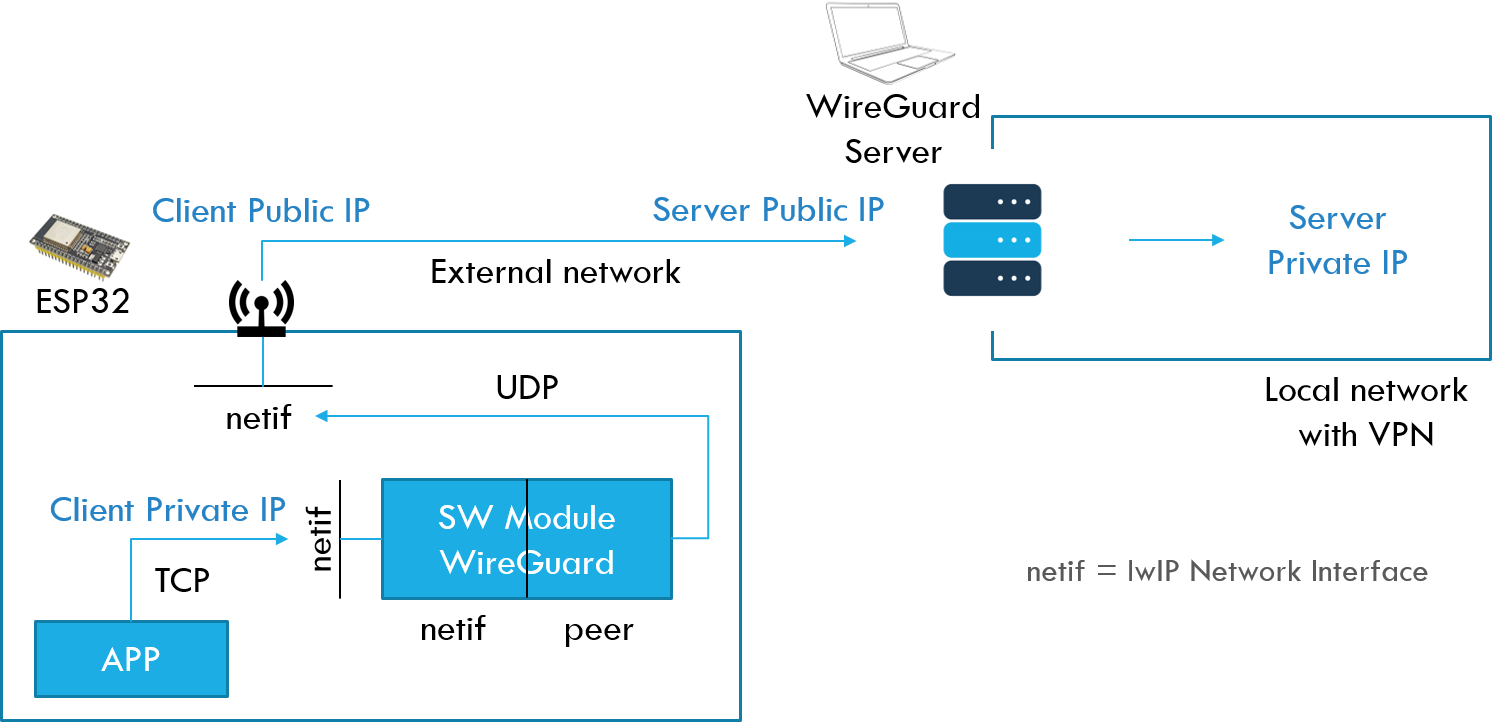
\includegraphics[width=\textwidth]{images/ESP32_whit_VPN.png}
    \caption{Connection between ESP32 and server through VPN.}
    \label{fig:ESP32withVPN} % This is the image label, with which you can refer to the image in any document location.
\end{figure}

